\section{堆排序}

\subsection{堆的实现}

我们一般采用完全二叉树实现堆,这样所有的操作都可以抽象在数组中完成,而不必使用链表。下面是一些概念重申:

\begin{itemize}
  \item 完全二叉树,除了最后一层外,其他各层结点数达到最大,最后一层所有的节点都集中在左侧的满二叉树。
  \item 有序: 二叉树每个节点都大于等于或小于等于其子节点(本节默认使用大根堆)。
\end{itemize}

二叉堆是一组有序的完全二叉树排列的元素,并在数组中按照层级存储(不使用数组第一个位置)。下面将二叉堆简称为堆。

二叉堆与数组下标的对应关系如下:

\begin{figure}[H]
    \small
    \centering
    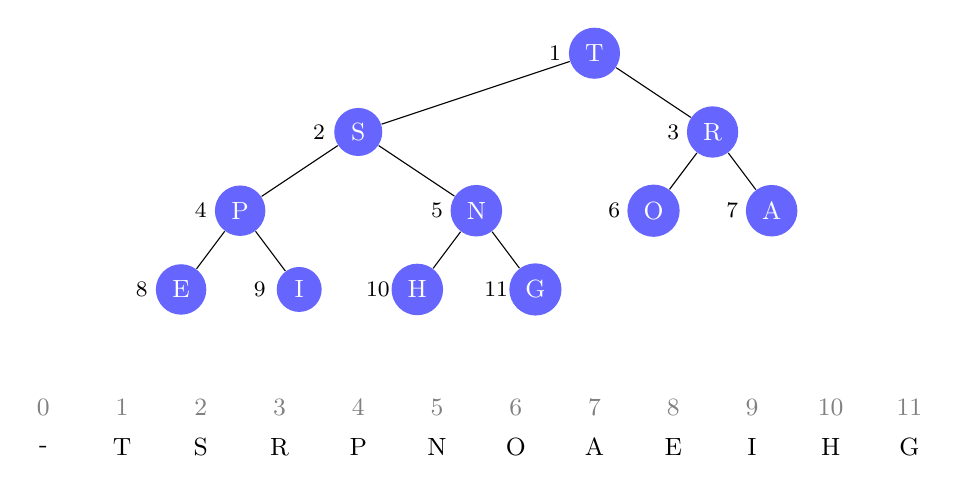
\begin{tikzpicture}[font=\small]
        \begin{scope}[color=white, circle]
            \node[fill=blue!60] (T) at (0,0) {T};
            \node[fill=blue!60] (S) at (-3,-1) {S};
            \node[fill=blue!60] (R) at (1.5,-1) {R};
            \node[fill=blue!60] (P) at (-4.5,-2) {P};
            \node[fill=blue!60] (N) at (-1.5,-2) {N};
            \node[fill=blue!60] (E) at (-5.25,-3) {E};
            \node[fill=blue!60] (I) at (-3.75,-3) {I};
            \node[fill=blue!60] (H) at (-2.25,-3) {H};
            \node[fill=blue!60] (G) at (-0.75,-3) {G};
            \node[fill=blue!60] (O) at (0.75,-2) {O};
            \node[fill=blue!60] (A) at (2.25,-2) {A};
            \draw[color=black] (T) -- (S);
            \draw[color=black] (T) -- (R);
            \draw[color=black] (S) -- (P);
            \draw[color=black] (S) -- (N);
            \draw[color=black] (R) -- (O);
            \draw[color=black] (R) -- (A);
            \draw[color=black] (P) -- (E);
            \draw[color=black] (P) -- (I);
            \draw[color=black] (N) -- (H);
            \draw[color=black] (N) -- (G);
        \end{scope}
        \begin{scope}[font=\footnotesize, xshift=-0.5cm]
            \node (T) at (0,0) {1};
            \node (S) at (-3,-1) {2};
            \node (R) at (1.5,-1) {3};
            \node (P) at (-4.5,-2) {4};
            \node (N) at (-1.5,-2) {5};
            \node (E) at (-5.25,-3) {8};
            \node (I) at (-3.75,-3) {9};
            \node (H) at (-2.25,-3) {10};
            \node (G) at (-0.75,-3) {11};
            \node (O) at (0.75,-2) {6};
            \node (A) at (2.25,-2) {7};
        \end{scope}
        \begin{scope}[yshift=-5cm, xshift=-7cm]
            \node (0) at (0,0) {-};
            \node (1) at (1,0) {T};
            \node (2) at (2,0) {S};
            \node (3) at (3,0) {R};
            \node (4) at (4,0) {P};
            \node (5) at (5,0) {N};
            \node (6) at (6,0) {O};
            \node (7) at (7,0) {A};
            \node (8) at (8,0) {E};
            \node (9) at (9,0) {I};
            \node (10) at (10,0) {H};
            \node (11) at (11,0) {G};
        \end{scope}
        \begin{scope}[yshift=-4.5cm, xshift=-7cm, color=gray]
            \node (0) at (0,0) {0};
            \node (1) at (1,0) {1};
            \node (2) at (2,0) {2};
            \node (3) at (3,0) {3};
            \node (4) at (4,0) {4};
            \node (5) at (5,0) {5};
            \node (6) at (6,0) {6};
            \node (7) at (7,0) {7};
            \node (8) at (8,0) {8};
            \node (9) at (9,0) {9};
            \node (10) at (10,0) {10};
            \node (11) at (11,0) {11};
        \end{scope}
    \end{tikzpicture}
    \caption{二叉堆与数组}
    \label{fig:二叉堆与数组}
\end{figure}

在二叉堆中我们会发现如下规律:
\begin{itemize}
  \item 第 k 个节点的子节点数组下标分别是 2k, 2k+1。
  \item 第 k 个节点的子节点数组下标是 k/2。
  \item 大小为 N 的完全二叉树高度为 $\lceil \log_2 N \rceil$
\end{itemize}

\subsection{堆的算法}

\subsubsection{堆上浮与下沉}

针对二叉堆的插入和删除操作对应两种算法:
\begin{itemize}
    \item 上浮: 某个节点优先级上升,我们需要由下至上恢复堆的顺序。
    \item 下沉: 某个节点优先级下降,我们需要由上至下恢复堆的顺序。
\end{itemize}

如果堆的有序状态因为某个结点变得比它的父结点更大而被打破,那么我们就需要通过交换它和它的父结点来修复堆。

二叉堆上浮非常简单,通过比较父节点(下标为 k/2)元素大小决定是否交换位置。
\begin{itemize}
    \item 由于可能存在的另一个子节点一定比父节点小,因此交换不会影响子节点。
    \item 由于父节点一定比子节点大,因此父节点被交换后仍然比孙节点大。
\end{itemize}

因此上浮只需要一直比较交换,直到到顶即可:

\begin{Java}
private static void swim(int k) {
    while (k > 1 && MathUtils.isLess(arr[k / 2], arr[k])) {
        CollectionUtils.exchange(arr, k / 2, k);
        k = k / 2;
    }
}
\end{Java}

如果堆的有序状态因为某个结点变得比它的两个子结点或是其中之一更小了而被打破了,那么我们可以通过将它和它的两个子结点中的\textbf{较大者}交换来恢复堆。

\begin{Java}
private static void sink(int k) {
    while (2 * k <= arr.length) {
        int j = 2 * k;
        if (j < arr.length && MathUtils.isBig(arr[j+1], arr[j]))
            j += 1;
        if (MathUtils.isLess(arr[j], arr[k])) break;
        CollectionUtils.exchange(arr, k, j);
        k = j;
    }
}
\end{Java}

上浮和下沉操作均不会改变二叉堆的有序性,利用这一点可以对二叉堆进行增删改操作。

有了上浮与下沉算法,插入与删除就变成十分简单:
\begin{itemize}
    \item 插入: 将元素插入到数组尾部,并对元素进行上浮。
    \item 删除: 仅能删除头部元素,然后将数组最后一个元素放到头部进行下沉。
    \item 修改: 改小进行下沉,改大进行上浮。
\end{itemize}

\subsubsection{优先队列}

由于数组第一个位置元素并不存储数据,我们可以用它来表示元素集合的长度。继而实现所有操作,我们可以得到一个优先队列:

\begin{Java}
public class MaxPQ<Key extends Comparable<Key>> {
    private Key[] pq;
    private int N = 0;

    public MaxPQ(int maxN) {
        pq = (Key[]) new Comparable[maxN + 1];
    }

    public boolean isEmpty() {
        return N == 0;
    }

    public int size() {
        return N;
    }

    public void insert(Key v) {
        pq[++N] = v;
        swim(N);
    }

    public Key delMax(Key v) {
        Key max = pq[1];
        pq[1] = pq[N--];
        pq[N + 1] = null;
        sink(1);
        return max;
    }

    private void swim(int k) {
        while (k > 1 && MathUtils.isLess(pq[k / 2], pq[k])) {
            CollectionUtils.exchange(pq, k / 2, k);
            k = k / 2;
        }
    }

    private void sink(int k) {
        while (2 * k <= pq.length) {
            int j = 2 * k;
            if (j < pq.length && MathUtils.isBig(pq[j++], pq[j]))
                j += 1;
            if (MathUtils.isLess(pq[j], pq[k])) break;
            CollectionUtils.exchange(pq, k, j);
            k = j;
        }
    }
}
\end{Java}

\subsection{堆排序}

前面我们已经知道了构建有序堆的具体算法,利用这种算法对数组进行排序只需如下两步:
\begin{itemize}
    \item 构造阶段: 将待排序的数组构造成一个大根堆,此时,最大值处于顶端。
    \item 排序阶段: 将顶端元素与末尾元素交换,此时最大值在数组尾部。将剩余 n-1 个元素重新构造成大根堆(顶端元素下沉), 重复该步骤。
\end{itemize}

\subsubsection{构造阶段}

首先,我们将数组看成完全二叉树,由于此时数组下标从 0 开始,因此下标为 k 的节点,其子节点 m 应该有如下关系:

$$ m+1 = 2(k+1) \text{或} 2(k+1)+1 $$

由此可以得出节点 k 的父子节点的关系:
\begin{itemize}
    \item 子节点: 2k+1, 2k+2
    \item 父节点: k/2 + k\%2 - 1
\end{itemize}

直到了这些关系后,我们从后往前找到最后一个非叶子节点,然后依次让所有非叶子节点下沉,就构建了一颗有序堆:
\begin{itemize}
    \item 最后一个非叶子节点位置: (N-1) 代入查父节点公式: $\frac{N-1}{2} + (N-1)\%2 -1 \le N/2$, 这里也可以通过长度奇偶分类,但单个叶节点下沉耗时可忽略不计,甚至不如不分类。
\end{itemize}

为什么选择下沉而不是从头开始上浮呢? 通过上面计算我们直到,从尾到头下沉只需要下沉一半的元素,因为叶节点无需下沉,而上浮需要几乎所有的元素上浮。

\subsubsection{排序阶段}

排序阶段的活就很简单了,首个元素与末尾元素交换,再让新的首个元素下沉,最后我们得到堆排序代码如下:

\begin{Java}
public static void heapSort(Comparable[] arr) {
    int N = arr.length;
    for (int i = N / 2; i >= 0; i--)
        sink(arr, i, N);
    while (N > 1) {
        CollectionUtils.exchange(arr, 0, --N);
        sink(arr, 0, N);
    }
}

private static void sink(Comparable[] arr, int k, int N) {
    while (2 * k + 1 <= N - 1) {
        int j = 2 * k + 1;
        if (j + 1 <= N - 1 && MathUtils.isBig(arr[j + 1], arr[j]))
            j++;
        if (MathUtils.isBig(arr[k], arr[j])) break;
        CollectionUtils.exchange(arr, k, j);
        k = j;
    }
}
\end{Java}

\subsection{算法评价}

\begin{itemize}
  \item 时间复杂度: $O(n\log_2 n)$。
  \item 空间复杂度: $O(1)$。
  \item 稳定性: 不稳定。
\end{itemize}

堆排序有着许多快速排序的优点: 无需额外空间,原地排序;同时兼具归并排序的稳定性。但是它有一个致命的缺陷,导致它的使用率远不及快排和归并排序: 它的缓存命中率极低。再堆排序中我们往往需要比较 2k,k/2 位置的数据,因此缓存命中率远不及前两种算法,甚至不如希尔排序。

\newpage